\documentclass[10pt,a4paper]{article}
\usepackage[utf8]{inputenc}
\usepackage{amsmath}
\usepackage[landscape,margin=1cm]{geometry}
\usepackage[english]{babel}
\usepackage{minted}
\usepackage{mathtools}
\usepackage{amssymb}

%-------------------------
\usepackage[default]{raleway}
\usepackage{fontawesome}
\usepackage[T1]{fontenc}

\usepackage{hyperref}
\usepackage{enumitem}
\usepackage{lipsum}

\usepackage{xcolor}
\definecolor{customcolor}{HTML}{616AC5}
\definecolor{alert}{HTML}{CD5C5C}
\definecolor{w3schools}{HTML}{4CAF50}
\definecolor{subbox}{gray}{0.60}
\definecolor{codecolor}{HTML}{FFC300}
\colorlet{xx}{customcolor}


%--------------------------Editor mode.

\usepackage
[citestyle=authoryear,
sorting=nty,	  		%Sorts bibliography by year, name, title
autocite=footnote, 		%Autocite command generates footnotes
autolang=hyphen, 		
mincrossrefs=1, 	
backend=biber]
{biblatex}

\DeclareFieldFormat{postnote}{#1}
\DeclareFieldFormat{multipostnote}{#1}
\DeclareAutoCiteCommand{footnote}[f]{\footcite}{\footcites}

\bibliography{literature}
%----------------------------------------
%--------------------------------------------------------------------------------
\usepackage{tcolorbox}

\tcbuselibrary{most,listingsutf8,minted}

\tcbset{tcbox width=auto,left=1mm,top=1mm,bottom=1mm,
right=1mm,boxsep=1mm,middle=1pt}

\newenvironment{mycolorbox}[2]{%
\begin{tcolorbox}[grow to left by=-1em,grow to right by=-1em,capture=minipage,fonttitle=\large\bfseries, enhanced jigsaw,boxsep=1mm,colback=#1!30!white,on line,tcbox width=auto, toptitle=0mm,colframe=#1,opacityback=0.7,nobeforeafter,title=#2]%
}{\end{tcolorbox}\\[0.2em]}

\newenvironment{subbox}[2]{%
\begin{tcolorbox}[capture=minipage,fonttitle=\normalsize\bfseries, enhanced jigsaw,boxsep=1mm,colback=#1!30!white,on line,tcbox width=auto,left=0.3em,top=1mm, toptitle=0mm,colframe=#1,opacityback=0.7,nobeforeafter,title=#2]\footnotesize %
}{\normalsize\end{tcolorbox}\vspace{0.1em}}

\newenvironment{multibox}[1]{%
\begin{tcbraster}[raster columns=#1,raster equal height,nobeforeafter,raster column skip=1em,raster left skip=1em,raster right skip=1em]}{\end{tcbraster}}

\newenvironment{textbox}[1]{\begin{mycolorbox}{customcolor}{#1}}{\end{mycolorbox}}

%-------------------------------
\newtcblisting{codebox}[2]{colback=codecolor!5,colframe=codecolor!80!black,listing only, 
minted options={numbers=left,style=tcblatex,fontsize=\tiny,breaklines,autogobble,linenos,numbersep=3mm},
left=5mm,enhanced,
title=#2, fonttitle=\bfseries,
listing engine=minted,minted language=#1}

%--------------------------------------------------------------------------------
\newcommand{\punkti}{~\lbrack\dots\rbrack~}

\renewenvironment{quote}
               {\list{\faQuoteLeft\phantom{ }}{\rightmargin\leftmargin}%
                \item\relax\scriptsize\ignorespaces}
               {\unskip\unskip\phantom{xx}\faQuoteRight\endlist}
               

%--------------------------------------------------------------------------------
\newcommand{\bgupper}[3]{\colorbox{#1}{\color{#2}\huge\bfseries\MakeUppercase{#3}}}
\newcommand{\bg}[3]{\colorbox{#1}{\bfseries\color{#2}#3}}

\newcommand{\mycommand}[2]{{\ttfamily\detokenize{#1}}~\dotfill{}~{\footnotesize #2}\\}
\newcommand{\sep}{{\scriptsize~\faCircle{ }~}}


\newcommand{\bggreen}[1]{\medskip\bgupper{w3schools}{black}{#1}\\[0.5em]}
\newcommand{\green}[1]{\smallskip\bg{w3schools}{white}{#1}}
\newcommand{\red}[1]{\smallskip\bg{alert}{white}{#1}}
\newcommand{\blue}[1]{\smallskip\bg{blue}{white}{#1}}
% Define
\definecolor{myblue}{RGB}{0,100,200}
\newcommand{\myblue}[1]{\smallskip\bg{myblue}{white}{#1}}


\usepackage{multicol}
\setlength{\columnsep}{5pt}

\setlength{\parindent}{0pt}
\pagestyle{empty}

\usepackage{csquotes}

\newcommand{\loremipsum}{Lorem ipsum dolor sit amet.}

%--------------------------------------------------------------------------------
\begin{document}
\small
\begin{multicols}{3}

    \scriptsize

    %----------Math Fundamentals Section ----------------
    \section{Math Fundamentals}
    \begin{textbox}{Formulae}
        \green{\emph{Asymptotics}} Let $f$ and $g$ be non-negative functions, then $f(n)$ is...\\

        \begin{tabular}{c|c|p{0.6\textwidth}}
                           & {\bf...if and only if...}                            & {\bf if $\lim\limits_{n \to \infty} \frac{f(n)}{g(n)}$} \\
            $O(g(n))$      & $\exists c,N:f(n)\leq c\cdot g(n)$ for $n\geq N$     & $\neq \infty$.                                          \\
            $o(g(n))$      & $\forall c,\exists N:f(n)\leq c\cdot g(n)$ for $n>N$ & $= 0$.                                                  \\
            $\Omega(g(n))$ & $\exists c,N:f(n)\geq c\cdot g(n)$ for $n\geq N$     & $\neq 0$                                                \\
            $\omega(g(n))$ & $\forall c,\exists N:f(n)\geq c\cdot g(n)$ for $n>N$ & $= \infty$.                                             \\
            $\Theta(g(n))$ & $f(n)$ is $O(g(n))$ and $g(n)$ is $O(f(n))$          & $\neq 0, \infty$                                        \\
        \end{tabular}\\
        \linebreak
        \begin{tabular}{c|p{0.8\textwidth}}
            {\bf Implications}                        & {\bf Equivalences}                                                  \\
            $f = o(g) \Rightarrow f = O(g)$           & $f = O(g) \Leftrightarrow g = \Omega(f)$                            \\
            $f = \omega(g) \Rightarrow f = \Omega(g)$ & $f = o(g) \Leftrightarrow g = \omega(f)$                            \\
                                                      & $f = O(g) \text{ and } f = \Omega(g) \Leftrightarrow f = \Theta(g)$ \\
        \end{tabular}
        \linebreak
        {\bf Generalizations:} For all $a, b > 0$, $k > 1$, and $n \geq 1$
        \[\begin{cases}
                (\log n)^b = o(n^a)                                                                 \\
                n^b = o((1 + a)^n)                                                                  \\
                a^{\sqrt{\log n}} = o(n^b)                                                          \\
                k^n > n! > n^{n^b} > n^a > \log n > n^{1/k} > O(1) & \text{ $\approx$ comparisions} \\
                n! \approx n^n \cdot e^{-n} \cdot \sqrt{2\pi n}    & \text{ Stirling's Formula }    \\
            \end{cases}\]
        \green{\emph{Master Theorem: }} Let $T(n) = aT(n/b) + cn^k$ for $a \geq 1, b \geq 2, c, k \geq 0$. Then $T(n)$ is
        \[\begin{cases}
                \Theta(n^k)          & \text{if $a < b^k$} \\
                \Theta(n^k \log n)   & \text{if $a = b^k$} \\
                \Theta(n^{\log_b a}) & \text{if $a > b^k$} \\
            \end{cases}\]
    \end{textbox}

    %-----
    \section{Graph Algorithms}
    \begin{textbox}{Depth First Search Algorithm}
        \green{DFS Algorithm} \myblue{Runtime:} $O(|V| + |E|)$ \\
        1. Goes as deep as possible in the graph then backtrack.\\
        2. (In-class algorithm) marks preorder and postorder numbers of each node.\\
        3. In a directed graphs, DFS will label edges as follows. No cross edges in undirected graphs.\\
        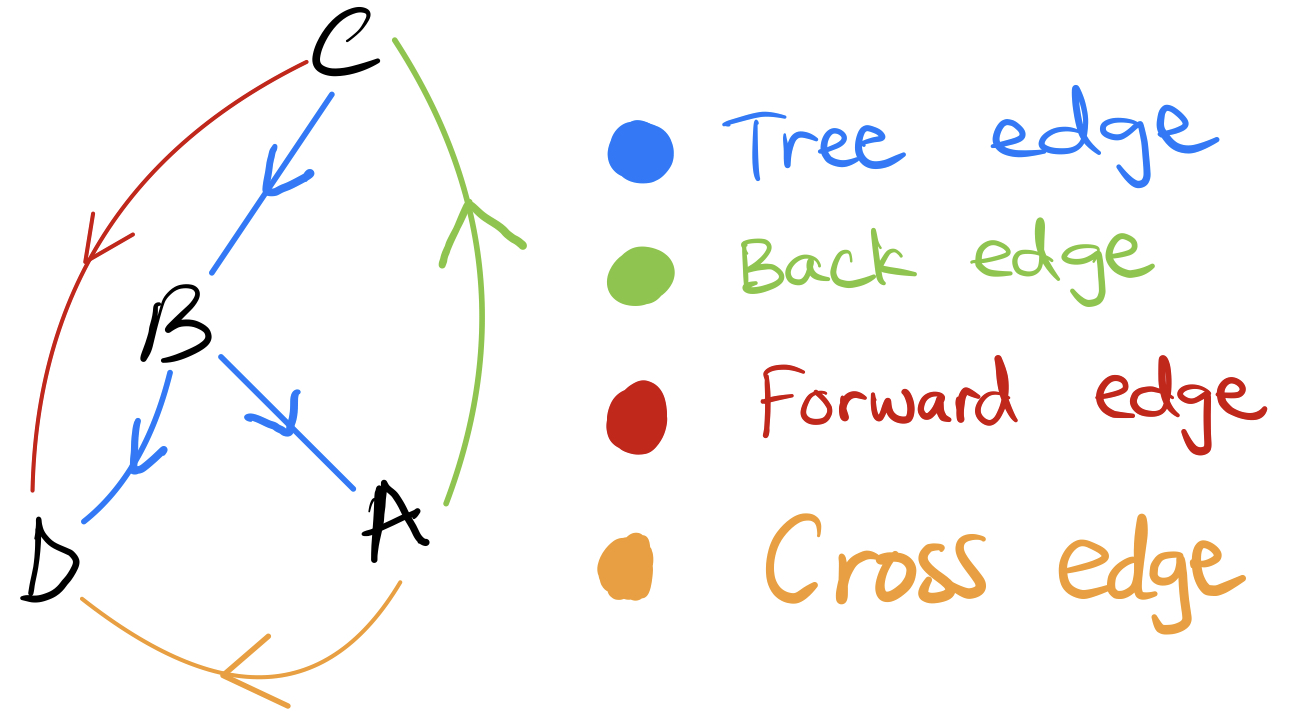
\includegraphics[width=0.4\textwidth]{images/dfs-edges.jpeg}\\
        \myblue{Applications:}\\
        \begin{tabular}{c|p{0.6\textwidth}}
            Detecting cycles               & $\exists$ (u, v): postorder(u) < postorder(v) \\
            Topological Sort on {\bf DAGs} & Decreasing post-order                         \\
            Strongly Connected Components  & Hint: DFS on reversed Graph.                  \\
        \end{tabular}\\
    \end{textbox}

    % ------------- Single Source Shortest Paths ----------------
    \begin{textbox}{Single Source Shortest Paths}
        %----- BFS Algorithm  ----------------
        \green{BFS Algorithm} \red{only for unweighted graphs.} \\
        1. Goes level by level in the graph.\\
        2. Uses a queue to process nodes.\\
        \myblue{Runtime:} $O(|V| + |E|)$ \\
        \linebreak
        Let  {\bf \textcolor{blue}{update(u, v)}} be defined as: if $Dist[u] + \text{length}(u, v)< Dist[v]$, update: $Prev[v] = u$ and $Dist[v] = Dist[u] + \text{length}(u, v)$.\\
        \green{Dijkstra’s Algorithm:} \red{only $+$ve weighted graphs} \\
        1. Let $Dist[v] = \infty$ and $Prev[v] = $ NIL for all vertices $v$.\\
        2. Let $Dist[s] = 0$ and initialize MinHeap with $(s, 0)$.\\
        3. While heap isn't empty, keep poping the vertex (say $u$) with the smallest distance. For each neighbor $v$ of $u$ with weight $w$, {\bf \textcolor{blue}{update(u, v)}}.\\
        \linebreak
        \myblue{Runtime:} $O(|V|*popMin + |E|*Insert)$ \\
        \linebreak
        \green{Bellman-Ford Algorithm:} \red{Only $+$ and $-$ve weighted graphs}\\
        1. Let $Dist[v] = \infty$ and $Prev[v] = $ NIL for all vertices $v$.\\
        2. Let $Dist[s] = 0$.\\
        3. For $|V|-1$ times: For each edge $(u, v)$, {\bf \textcolor{blue}{update(u, v)}}\\
        4. Checking for negative weight cycles: repeat the above step once. If any distance can still be improved, a negative weight cycle exists. Hence, return {\bf Inconclusive}\\
        \linebreak
        \myblue{Runtime:} $O(|V|*|E|)$ \\
        \linebreak
        \green{Linear Runtime:} \red{only for Directed Acyclic Graphs (DAGs)} \\
        1. Run DFS to get topological sort.\\
        2. For every edge ($u, v$), in topological sort, {\bf \textcolor{blue}{update(u, v)}}.\\
        \myblue{Runtime:} $O(|V| + |E|)$ \\
    \end{textbox}

    \begin{textbox}{Min Heaps}
        \green{Representation:} Visually a complete tree. Implementationwise,\\
        let $A[0..n-1]$ be a list where $A[0]$ is the root and for any $i$th element, its parent, left, and right children are at $\lfloor i/2 \rfloor, 2i, 2i+1$ respectively.\\
        \linebreak
        {\bf \emph{Heap Property:}} The parent element is smaller than its children.\\
        \linebreak
        \begin{tabular}{c |p{0.7\textwidth}}\scriptsize
            {\bf Operations} & {\bf Description}                                                                  \\
            $Insert(a)$      & let $A[n] = a$ and $HeapifyUp(n)$                                                  \\
            $PopMin$         & let $A[0] = A[n-1]$ and $HeapifyDown(0)$                                           \\
            $HeapifyUp(i)$   & repeatedly swap $A[i]$ with its parent until the heap property is restored         \\
            $HeapifyDown$    & repeatedly swap $A[i]$ with its smallest child until the heap property is restored \\
        \end{tabular}
        \myblue{Heaps Operations and Runtimes:} Both $O(\log n)$ with binary heaps. \\
        \red{Note:} Can do better with Fibo-Heaps (amortized $O(1)$ for PopMin.)\\
    \end{textbox}



    %-------------Minimum Spanning Trees ----------------

    \begin{textbox}{Minimum Spanning Trees}
        \blue{Basic Properties:}
        \begin{enumerate}
            \item {\bf a Tree} is connected, acyclic, and has $|V|-1$ edges (any two implies the third).
            \item {\bf Cut Property} states that for any cut of a connected, undirected graph, the minimum weight edge that crosses the cut belongs to the MST.
            \item Only for connected, undirected, and weighted (non-negative) graphs.
        \end{enumerate}
        \green{Prim's Algorithm:}
        \begin{enumerate}
            \item Start with a single vertex and greedily add closest vertices.
            \item Similar to Dijkstra's algorithm, but $dist[v]$ is the weight of the edge connecting $v$ to the MST instead of the distance from $s$.
        \end{enumerate}
        \myblue{Runtime:} $O(|E| \log |V|)$ with Fibo-heaps\\
        \linebreak
        \green{Kruskal’s Algorithm:}\\
        1. Sort edges in ascending order of weight. \\
        2. Repeatedly add the lightest edge that does not create a cycle until we have $|V|-1$ edges.\\
        \linebreak
        \myblue{Runtime:} $nT(\text{Union}) + mT(\text{Find}) + T(\text{Sort $m$ Edges})$.\\
        \red{Notes:} Implemented using a union-find data structure.
    \end{textbox}


    \begin{textbox}{Disjoint Forest Data Structure}
        Maintain disjoint sets that can be combined ("unioned") efficiently. Operations MakeSet($x$), Find($x$), and Union($a, b$)\\
        \linebreak
        \myblue{Runtime:} Any sequence of $m$ UNIONs and $n$ FINDs operations take $O((m + n) \log^* n)$.\\
        \red{Note:} $\log^* n$ is the number of times we can $\log_2$ $n$ until we get $\leq$ 1.\\
        \red{Heuristics:}
        \begin{itemize}
            \item Union by rank. When performing a union operation, we prefer to merge the shallower tree into the deeper tree.
            \item Path compression. After performing a find operation, attach all the nodes touched directly onto the root of the tree.
        \end{itemize}
        \green{Example:}\\
        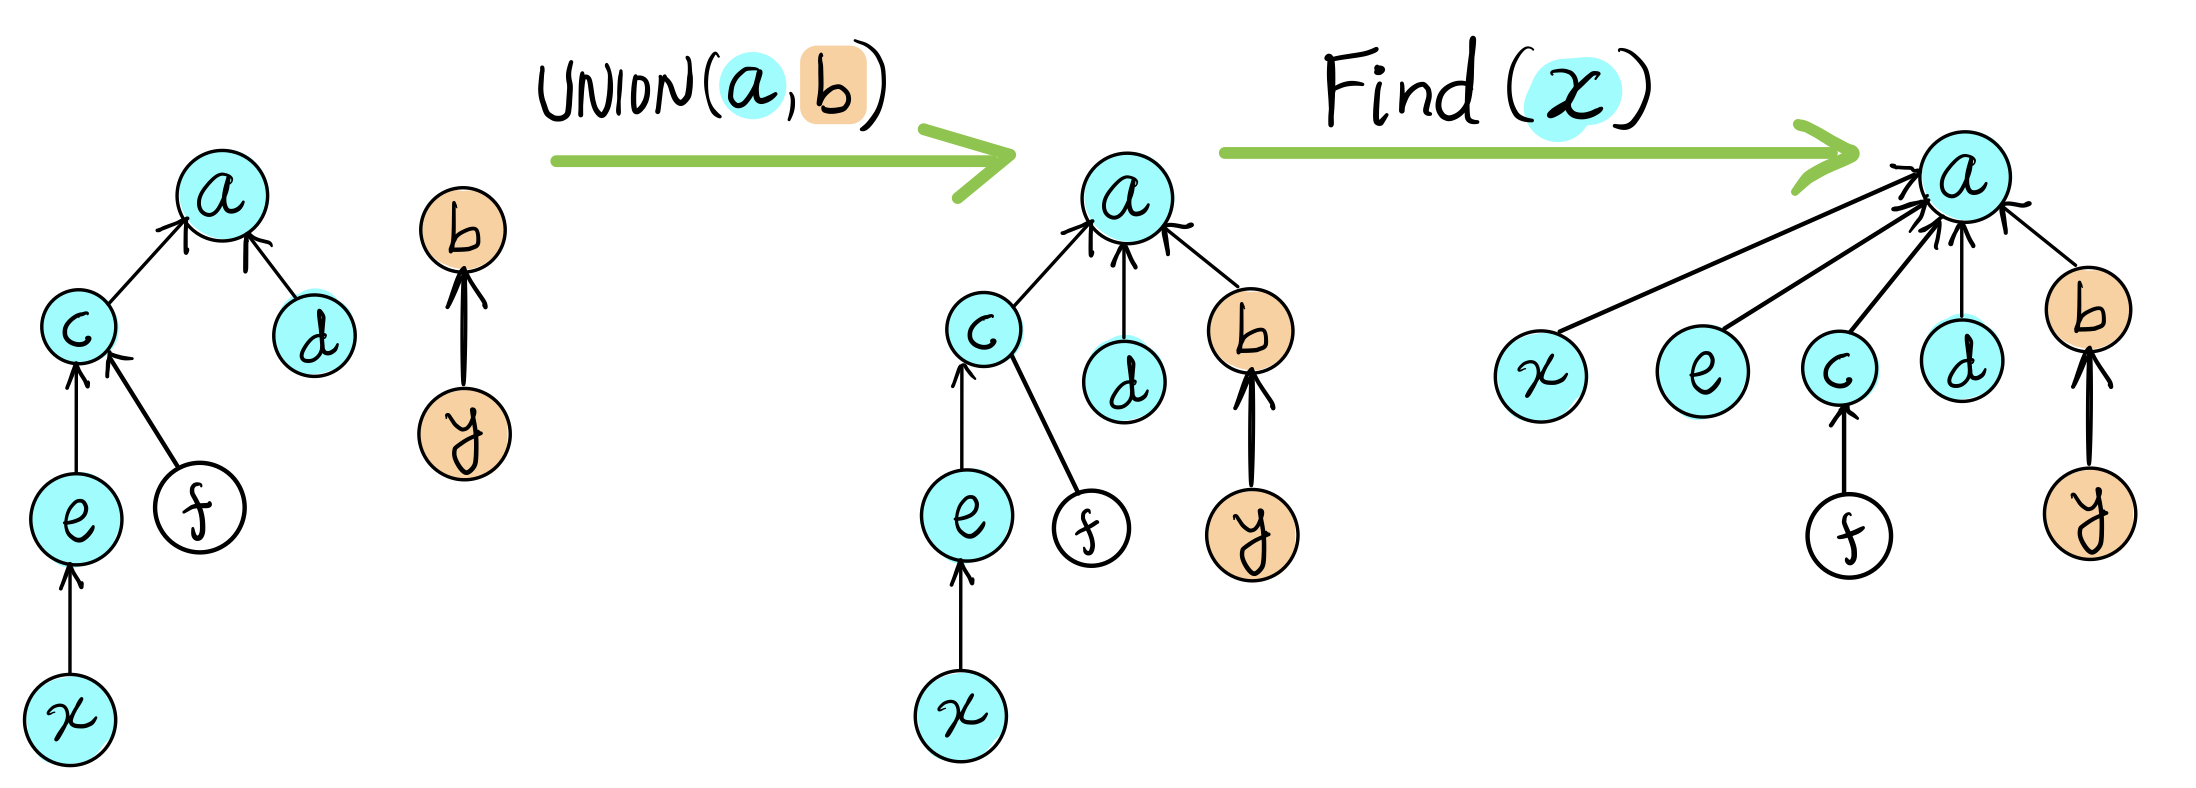
\includegraphics[width=\textwidth]{images/Union-Find.jpeg}
    \end{textbox}

    %-------------Greedy Algorithms ----------------
    \section{Greedy Algorithms}

    \begin{textbox}{}
        \green{Main idea:} At each step, make a locally optimal choice in hope of reaching the globally optimal solution. \\
    \end{textbox}
    \begin{textbox}{Horn Formula}
        \green{Algorithm:} Set all variables to false and greedily set ones to be true when forced to.\\
        \linebreak
        \myblue{Runtime:} linear time in the length of the formula (i.e., the total number of appearances of all literals). \\
        \linebreak
        \red{Notes:} Only works for SAT instances where in each clause, there is at most one positive literal.
    \end{textbox}

    \begin{textbox}{Huffman Coding}
        \green{Algorithm:} \myblue{Runtime:} $O(n\log n)$ \\
        Find the best encoding by greedily combining the two least frequently items. Optimal in terms of encoding one character at a time.\\
        \linebreak
        \red{Example:} A Huffman tree for string  "Mississippi River"\\
        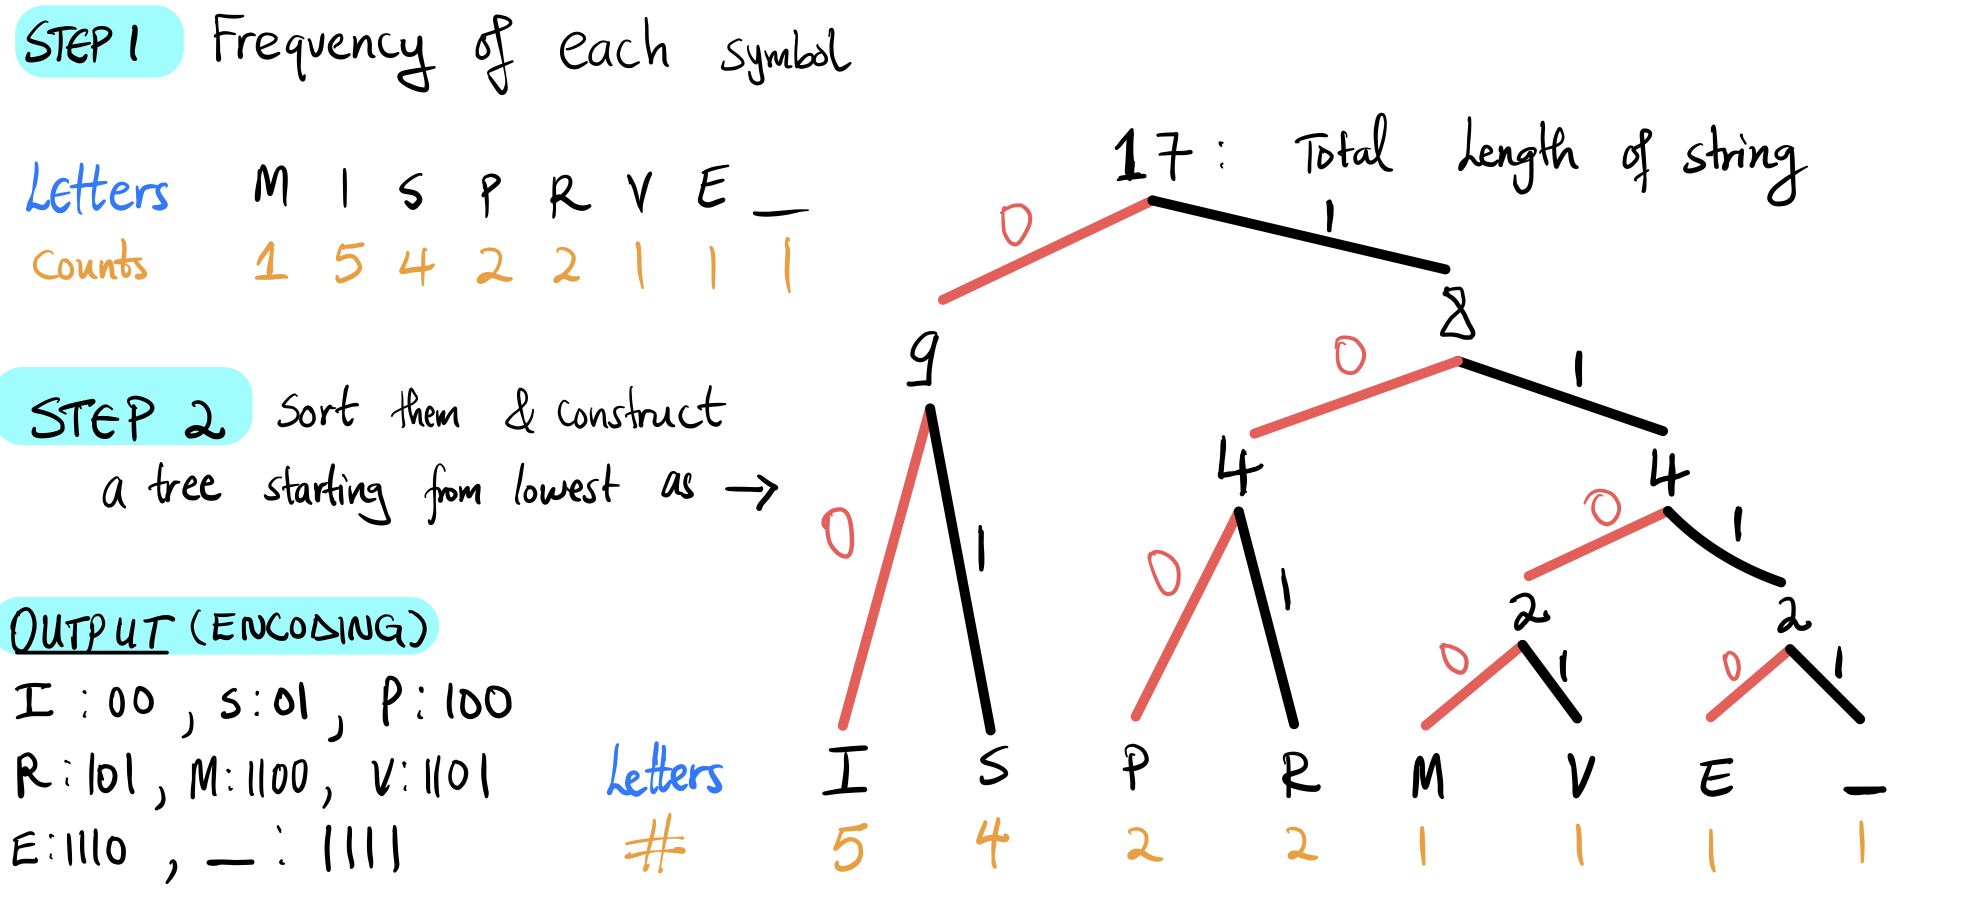
\includegraphics[width=0.75\textwidth]{images/Huffman-coding.jpeg}
    \end{textbox}

    \begin{textbox}{Set Cover}
        Given $X = \{x_1,\ldots,x_n\}$, and a collection of subsets $\cal{S}$ of $X$ such
        that $\bigcup_{S \in \cal{S}} S = X$, find the subcollection $\cal{T} \subseteq \cal{S}$ such that the sets of
        $\cal{T}$ cover $X$.\\
        \linebreak
        \green{Algorithm:} \myblue{Runtime:} $O(|U|)$ \\
        1. Greedily choose the set that covers the most number of the remaining uncovered elements at the given iteration.\\
        {\bf claim:} Let $k$ be the size of the smallest set cover for
        the instance $(X,\cal{S})$.  Then the greedy heuristic finds
        a set cover of size at most $k \ln n$.
        \linebreak
        \red{Note:}\\Not always optimal; achieves $O(\log n)$ approximation ratio.
    \end{textbox}

    %-------------Divide and Combine ----------------
    \section{Divide and Combine}

    \begin{textbox}{}
        \green{Main Idea:} Divide the problem into smaller pieces, recursively solve those, and then combine their results to get the final result.\\
    \end{textbox}

    \begin{textbox}{Famous Examples w/ Runtimes}
        \begin{tabular}{r|p{0.8\textwidth}}\scriptsize
            Mergesort              & $O(n\log n)$                                     \\
            Min and Max on a line  & $\frac{3}{2}n - 2$ comparisions; $O(n)$ runtime. \\
            Closest Pair of Points & $O(n \log^2 n)$                                  \\
        \end{tabular}
    \end{textbox}

    \begin{textbox}{$n$-digit Integer Multiplication}
        \begin{tabular}{r|p{0.8\textwidth}}\scriptsize
            standard Multiplication    & $\Theta(n^2)$                             \\
            3 products on $n/2$ digits & $\Theta(n^{\log_2 3}) = \Theta(n^{1.59})$ \\
            5 products on $n/3$ digits & $\Theta(n^{\log_3 5}) = \Theta(n^{1.46})$ \\
        \end{tabular}
        \linebreak
    \end{textbox}

    \begin{textbox}{$n \times n$ Matrix Multiplication}
        \green{Strassen's Algorithm:} \myblue{Runtime:} $O(n^{\log_2 7})$ \\
        Divide into four submatrices, each of size $n/2$ by $n/2$.
        $$
            \left[ \begin{array} {cc} A & B \\ C & D \end{array} \right ]
            \left[ \begin{array} {cc} E & F \\ G & H \end{array} \right ]
            =
            \left[ \begin{array} {cc} AE+BG & AF+BH \\ CE+DG & CF+DH \end{array} \right ]
        $$
        Find: $P_1 = A(F-H)$, $P_2 = (A+B)H$, $P_3 = (C+D)E$, $P_4 = D(G-E)$, $P_5 = (A+D)(E+H)$, $P_6 = (B-D)(G+H)$, $P_7 = (C-A)(E+F)$, then: \\
        \linebreak
        $AE+BG = -P_2 + P_4 + P_5 + P_6$ and $AF +BH = P_1 + P_2$\\
        $CE+DG = P_3 + P_4$ and $CF +DH = P_1 - P_3 + P_5 + P_7$\\
    \end{textbox}

    %-------------Dynamic Programming ----------------
    \section{Dynamic Programming}

    \begin{textbox}{}
        \green{Main Idea:} Maintain a lookup table of correct solutions to sub-problems and build up this table towards the actual solution.\\
        \blue{Steps:}
        \begin{enumerate}
            \item Define subproblems and recurrence to solve subproblems.
            \item Combine with {\bf reuse}.
            \item Runtime and space analysis.
        \end{enumerate}
    \end{textbox}

    \begin{textbox}{\href{https://leetcode.com/problems/edit-distance/}{Edit Distance}}
        Find the minimum number of operations required to transform one string, $A[1\ldots n]$, into another, $B[1\ldots m]$. \\
        \green{Algorithm:} \myblue{Runtime and Space:} $O(nm)$
        \begin{enumerate}
            \item Subproblem: let $D(i,j)$ represent the edit distance between $A[1\ldots i]$ and $B[1\ldots j]$.
            \item Recurrence is: \\
                  Base cases: $D(i,0) = i, D(0,j) = j.$ \\
                  $D(i,j) = \min[D(i-1,j)+1,D(i,j-1)+1,D(i-1,j-1)+ (1 \text { if } i = j \text {, $0$ otherwise})].$
            \item return $D(n,m)$.
        \end{enumerate}
    \end{textbox}

    \begin{textbox}{All Pairs Shortest Paths}
        Given a graph $G$ with $n$ vertices and $m$ edges, calculate distances of the shortest paths between {\em every} pair of nodes. \\
        \green{Floyd-Warshall Algorithm:} \myblue{Runtime:} $O(n^3)$
        \begin{enumerate}
            \item Subproblem: let $D_k[i,j]$ represent the shortest path between $i$ and $j$ using only nodes in $[1\ldots k]$.
            \item Recurrence is:
                  \[\begin{cases}
                          D_0[i,j] = d_{ij} \text{ if } i \text{ and } j \text{ are connected, } \infty \text{ otherwise}. \\
                          D_k[i,j] = \min(D_{k - 1}[i,j], D_{k - 1}(i,k)+D_{k - 1}[k,j]).
                      \end{cases}\]
            \item return $D(i,j,n)$.
        \end{enumerate}
        \red{Notes:} Does not work for cyclic graphs.
    \end{textbox}

    \begin{textbox}{Hashing and Set Resemblance}
        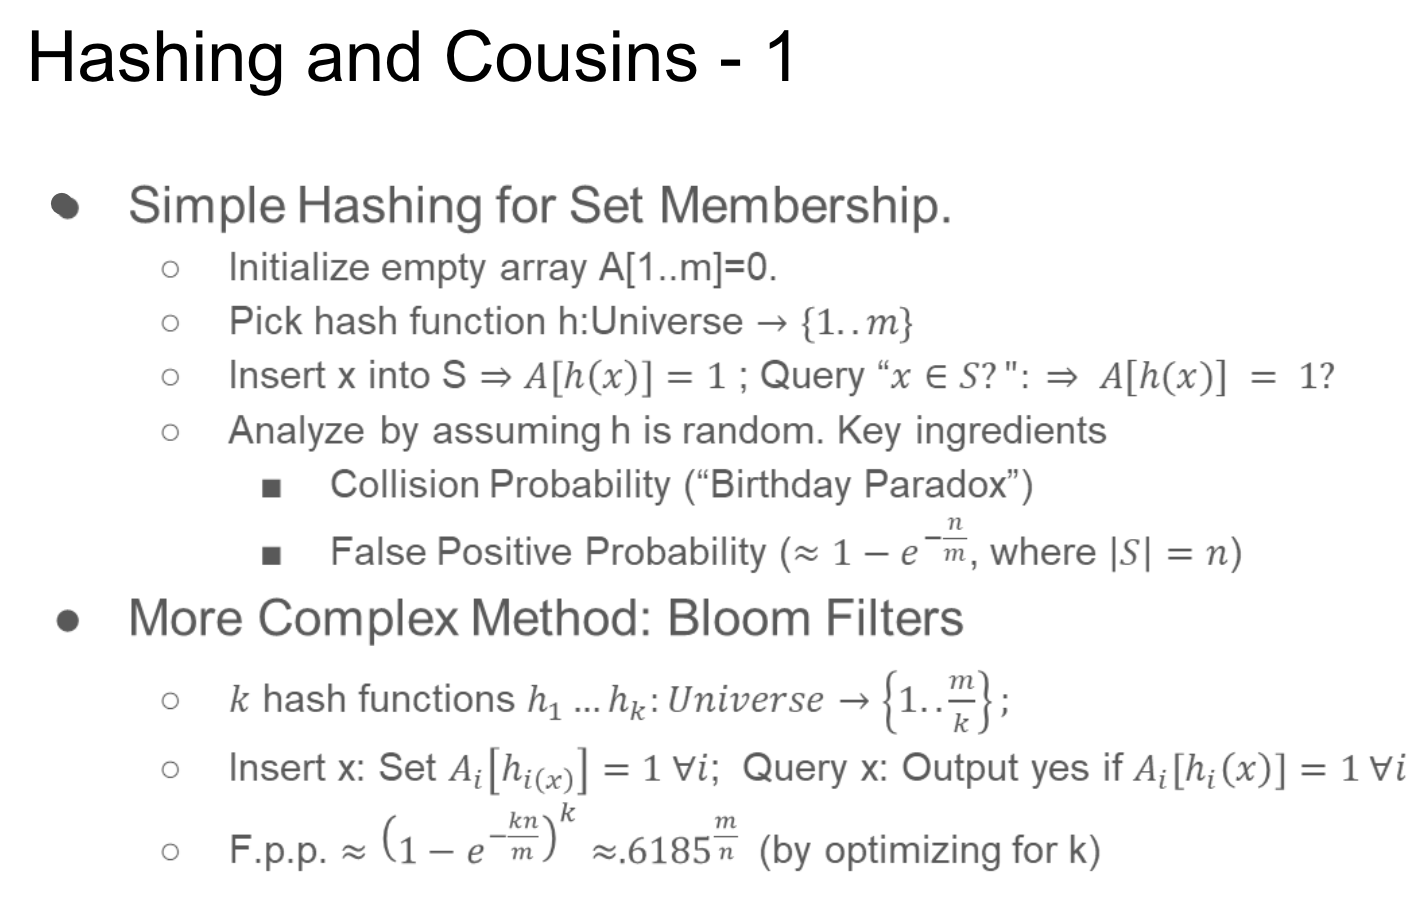
\includegraphics[width=0.7\textwidth]{images/Hashing1.png}

        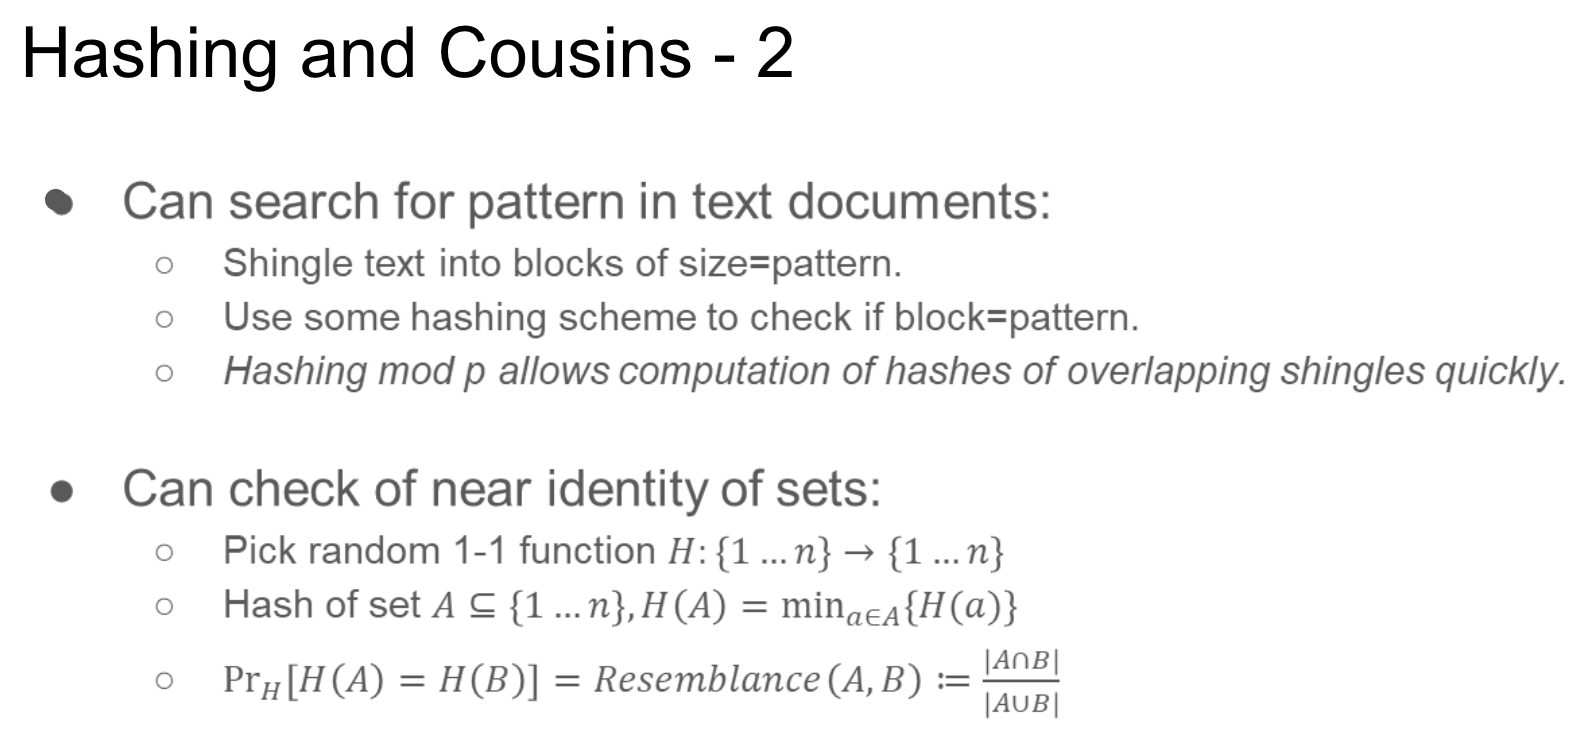
\includegraphics[width=0.7\textwidth]{images/Hashing2.png}


    \end{textbox}

    \begin{textbox}{Primality Testing}
        \green{Algorithm:} Generate large (d-digit) primes:
        Generate a random d-digit number, Check if it is prime, If not, repeat.\\

        Facts 1: $k^{th}$ prime number is $\Theta (k \log k)$.\\
        Fact 2: of the integers $1, \dots, n$, $\Theta(n/\log n)$ are prime.\\
        How many d-digits generations until prime: $O(d)$.

        \green{Fermat's Little Theorem:} \\
        If $p$ is prime and $a$ is not divisible by $p$, then $a \in \mathbb{Z}$, $a^{p-1} \equiv 1 \pmod{p}$.\\
        \red{Notes:}
        {\bf $a$-Pseudoprime $p$}: $a^{p-1} \equiv 1 \pmod{p}$, but $p$ is not prime.\\
        {\bf Carmichael number:} composite number $n$ s.t $a^{n-1} \equiv 1 \pmod{n}$ for all $a \in \mathbb{Z}$. Example: $561$ \\

        \green{Miller-Rabin Primality Test:} \\
        If $p$ is prime, the only solutions to $a^2 \equiv 1 \bmod p$ are $a \in \{\pm 1\}$. \\
        A {\bf non-trivial square root of 1} is an integer $a$ such that $a^2 \equiv 1 \pmod{n}$ and $a \not\equiv \pm 1 \pmod{n}$.\\
        \blue{The Test}
        \begin{enumerate}
            \item Choose a random $a \in [n]$
            \item \textcolor{purple}{if $a^{n-1} \not\equiv 1 \pmod{n}$, return $n$ is composite and $a$ is a witness.}
            \item Let $n-1 = 2^tu$ and compute $a^u, a^{2u},\ldots, a^{2^tu}$.
            \item Check for $a^{2^{i-1}u} \not\equiv \pm 1 \pmod{n}, a^{2^iu} \equiv 1 \pmod{n}$
            \item If so, we've found a {\em non-trivial square root} of 1 modulo $n$.
        \end{enumerate}
        $a$ is a {\bf witness} to the compositeness of $n$, if $n$ fails the test under $a$.\\
        \red{Note:} Let ${\bf F}$ be \textcolor{purple}{incorrectly} identifying $n$ as prime.  ${\bf Pr(F) \leq 1/4}$. With $k$ independent tests, $ {\bf Pr(F) \leq 4^{-k}}$.

        \blue{Operation Runtimes:}
        \begin{itemize}
            \item Most of these arthmetic operation has fast
                  polynomial runtime in $n$: addition, subtraction, multiplication, division, exponentiation, modular reduction, Euclid's algorithm, and Primality testing.
            \item \textcolor{red}{Exception:} Factor($a$): output all prime factors of $a$.
        \end{itemize}


    \end{textbox}

    \begin{textbox}{Euclid's algorithm \& RSA Cryptosystem}
        Def: $gcd(a, b) = max(d \in \mathbb{Z} : d | a \text{ and } d | b)$.\\
        \green{Basic algorithm:} find the $gcd(a, b)$ by repeatedly subtracting the smaller number from the larger number.\\
        \linebreak
        \green{Extended Euclid's algorithm:} find $x, y$ such that $ax + by = gcd(a, b)$.\\
        \begin{lstlisting}[language=Python]
        def gcd(a, b):      # a >= b >= 0
            if b == 0:
                return a
            return gcd(b, a mod b)
    \end{lstlisting}

        \begin{lstlisting}[language=Python]
        def Extended-Euclid(a,b): 	# a >= b >= 0
	        if b==0: return (a,1,0)
            Compute k such that a = bk + (a mod b)
            (d,x,y) = Extended-Euclid(b, a mod b)
            return (d,y,x-ky)

    \end{lstlisting}
        \blue{Example:} Find integers $x$ and $y$ such that $1240 x + 121 y = 1$.\\

        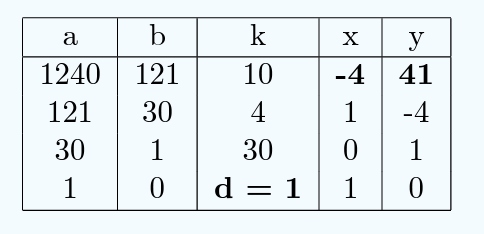
\includegraphics[width=0.5\textwidth]{images/ExtendedEuclid.png}

        \green{RSA Cryptosystem:} \\
        \blue{Receiver:} picks two large prime numbers $p$ and $q$, compute $n = pq$.
        Also, Picks $0 \le e \le n$ such that $gcd(e, (p-1)(q-1)) = 1$.
        \begin{itemize}
            \item \underline{private key:}
                  $${\bf d} = e^{-1} \pmod{(p-1)(q-1)}$$
                  $$\implies de \equiv 1 \pmod{(p-1)(q-1)}$$
            \item \underline{public key:} $(n, e)$
        \end{itemize}

        \green{RSA algorithm:} Let sender's message be $m$.
        \begin{enumerate}
            \item Encrytpion: $y = E(m) = m^e \pmod{n}$ —using public key $(n, e)$
            \item Decryption: $m = D(y) = y^{d} \pmod{n}$ —using private key $d$
        \end{enumerate}
    \end{textbox}


    \begin{textbox}{NP-c approximations}
        {\bf ${\bf \alpha}$-approximation:} $f$ is an $\alpha$-approximation to
        $f^*$ if $f(x) \leq \alpha f^*(x)$ for all $x$.

        \green{Independent Set:} Given a graph $G = (V, E)$, find largest set of
        vertices $S \subseteq V$ such that no two vertices in $S$ are adjacent.

        \green{Vertext Cover:} Given a graph $G = (V, E)$, find the smallest set of
        vertices $S \subseteq V$ such that every edge in $E$ is incident to at
        least one vertex in $S$.

        \green{Max Cut:} Given a graph, divide vertices into two sets to maximize
        number of edges between them.
        \begin{itemize}
            \item Split vertices arbitrarily.
            \item While moving a vertex impoves the solution, move it.
            \item stop when no more moves improve the solution.
        \end{itemize}
        \green{MAX SAT: Linear Relaxation}
        \begin{itemize}
            \item Convert formula to integer equations. E.g. $(X \vee
                      \bar{Y}) \to$ $x' + (1 - y') \geq 1$.
            \item Relax the constraint for variables $x', y', \dots \in \{0, 1\}$ to
                  $x', y', \dots \in [0, 1]$.
            \item Solve the relaxed problem to get assignment $x', y', \dots$
                  Then let $X = 1$ with probability $x'$
        \end{itemize}
        \blue{Claim:} If formular is satisfiable, then the number of clauses satisfied
        by above algorithm $\geq \text{ |clauses|} \cdot (1 - 1/e) \approx 0.63\text{ |clauses|}$

        \green{MAX SAT: Local Search}
        \begin{itemize}
            \item Pick a random assignment $x, y, \dots \in \{0, 1\}$.
            \item While moving a variable improves the solution, move it.
            \item stop when no more moves improve the solution.
        \end{itemize}
    \end{textbox}


    \begin{textbox}{Randomized 3-SAT Algorithm}
        {\bf Algorithm:} \underbar{Input:} a satisfiable 3SAT Formula with $n$ variables.
        \begin{itemize}
            \item Repeat:
                  \begin{enumerate}
                      \item Start with a random assignment of variables.
                      \item Do the following $3n$ times:
                            \begin{enumerate}
                                \item Check for an unstatisfied clause. If there is one, flip a random variable in that clause.
                                \item If the assignment satisfies all clauses, return the assignment.
                            \end{enumerate}
                  \end{enumerate}
        \end{itemize}

        {\bf Expected Runtime Analysis:}
        \begin{enumerate}
            \item Since in each flip we have $\frac{1}{2}$ probability of increasing
                  the score and $\frac{2}{3}$ of decreasing it. We can model this as the gambler's ruin problem.
                  the probability of finding a satisfying assignment will be $\Omega(c^n)$,
                  for some $c > 1/2$.
            \item The number of trials until a success is $\sim \text{FS}(O(c^n))$
                  giving us an expected number of trials equal to $O(c^{-n})$.
            \item In each trial, the algorithm do $3n$ steps, $O(3n)$, each of which
                  it checks all clauses. Since the are $n$ variables and each clauses can
                  have atmost $3$ variables, the number of unique clauses is $O(n^3)$.
            \item Resulting in a Expected runtime of $O(3n^4 c^{-n}) = o(2^{n})$.

        \end{enumerate}
    \end{textbox}

    \begin{textbox}{Network Flow}
        {\bf Story:} Given the number of available tickets $t_{ij}$ between cities
        $i$ and $j$, along with the city map, the goal is to maximize the number of
        tickets sold for people traveling from city $s$ to city $t$.

        \green{Reduction to LP:}
        \textbf{Objective function:}

        Maximize the total flow of tickets from the source node $s$ to the target node $t$. In other words, maximize the sum of $x_{st}$ over all edges $(s, t)$.

        \begin{equation}
            \text{maximize} \sum_{(s, t)} x_{st}
        \end{equation}

        \textbf{Subject to the following constraints:}

        1. Flow conservation constraints: For each node $i$, other than $s$ and $t$, the flow into the node must equal the flow out of the node.

        \begin{equation}
            \sum_{j} x_{ij} - \sum_{k} x_{ki} = 0, \forall i \neq s, t
        \end{equation}

        2. Capacity constraints: The flow of tickets on each edge $(i, j)$ must not exceed the available tickets $t_{ij}$.

        \begin{equation}
            0 \le x_{ij} \le t_{ij}, \forall (i, j)
        \end{equation}
        \green{Ford Fulkerson:}
        \begin{itemize}
            \item Make a Residual graph and Start with empty flow.
            \item While there is an augmenting path from $s$ to $t$:
                  \begin{itemize}
                      \item Find the bottleneck capacity $b$ on the path.
                      \item Increase the flow on the path by $b$ and update residues.
                  \end{itemize}
            \item The final flow is the maximum flow.
        \end{itemize}
        \textcolor{blue}{{\bf Augmenting path:}} is a path from $s$ to $t$ such that the flow on the path can be increased by at least one unit.

        \textcolor{blue}{{\bf Residual Graph:}}  for every edge (x,y) of G, add edge (y,x), capacity c(y,x) = flow f(x,y)

        \myblue{Runtime: }
        \begin{itemize}
            \item with DFS to find augmenting paths$O(VEU)$, where U is max edge capacity.
            \item $O(VE^2)$ with BFS (“Edmonds-Karp algorithm”).
        \end{itemize}

        \textcolor{blue}{{\bf Max-flow min-cut theorem:}} The maximum flow is equal to the minimum capacity of an $s$-$t$ cut.

        \smallskip
        Claim: when* Ford-Fulkerson terminates, we can find a cut matching the flow.
        \begin{itemize}
            \item No s-t path (of nonzero edges) in residual graph.
            \item Choose V1 = {vertices reachable from s}
            \item All edges e leaving V1 have f(e) = c(e)
            \item All edges e entering V1 have f(e) = 0
            \item So, total flow = capacity of cut.
        \end{itemize}

    \end{textbox}

    %--------------------------------------------- 
\end{multicols}
\end{document}

% \begin{enumerate}
%     \item Context-free grammar parsing $O(n^3m^2)$
%     \item DP on trees: Dominating Set   
%     \item Traveling salesman problem 
% \end{enumerate}